%! TEX program = lualatex
\documentclass[a4paper,11pt,onecolumn,twoside,openright,dvipsnames,%
%draft % for faster compiling comment-out this line and comment the 'final' line
final
]{memoir}

\usepackage{microtype} % better typography

% Math and physics packages
\usepackage{amsmath,amsthm}
% we don't load amssymb,amsfonts since we use unicode-math. load unicode-math AFTER amsmath,amsthm.
\usepackage{braket} % for Dirac notation

% Encoding and fonts
\usepackage{fontspec}
\usepackage{unicode-math}
\setmainfont{Libertinus Serif}
\setsansfont{Libertinus Sans}
\setmathfont{Libertinus Math}
\setmathfont[version=bold, FakeBold=2.5]{Libertinus Math}

\usepackage{adjustbox} % adjust tables, figures, etc

\usepackage{mleftright}
\mleftright % Makes \left and \right behave like \mleft and \mright document-wide

% Graphics
\usepackage{xcolor}
\usepackage{graphicx}
\graphicspath{{images/}}

\usepackage{tikz}
\usetikzlibrary{
    calc, 3d, shapes.geometric, arrows.meta, 
    decorations.markings, decorations.pathmorphing, 
    circuits.logic.US, circuits.ee.IEC, 
    positioning, shapes.gates.logic.US
}
\usetikzlibrary{external}
% Configure TikZ to use lualatex instead of pdflatex for the external images
\tikzset{external/system call={lualatex \tikzexternalcheckshellescape -halt-on-error -interaction=batchmode -jobname "\image" "\texsource"}}
% Set path for TikZ generated PDFs
\tikzexternalize[prefix=images/tikz/]


% Hyperlinks
\usepackage[linktocpage=true,colorlinks=false,linkbordercolor={RedViolet},urlbordercolor={cyan}]{hyperref}

% Add subsections to ToC and to add numbering to subsections
\setcounter{tocdepth}{4}
\setsecnumdepth{subsection}


% Custom math environments commands

% Use these commands instead of the symbols ", . ;" in math mode
\newcommand{\comma}{\,,}
\newcommand{\period}{\,.}
\newcommand{\semicolon}{\,;}

% Use with align* environment to print equation numbers in specific lines
\newcommand\numberthis{\addtocounter{equation}{1}\tag{\theequation}}

% Parentheses in math mode instead of \left and \right
\newcommand{\parentheses}[1]{\left( #1 \right)}
\newcommand{\sparentheses}[1]{\left[ #1 \right]}
\newcommand{\cparentheses}[1]{\left\{ #1 \right\}}


% Custom theorem environments
\newtheorem{theorem}{Theorem}[chapter]
\newtheorem{definition}{Definition}[chapter]
\newtheorem{axiom}{Postulate}
\newtheorem{remark}{Remark}[chapter]
\newtheorem{sproblem}{Solved Problem}[chapter]
\newtheorem{problem}{Problem}[chapter]


% Bibliographic references
\usepackage[backend=biber,sorting=none,bibstyle=numeric,citestyle=numeric-comp,url=false,
  eprint=true,isbn=false,doi=false,maxbibnames=5]{biblatex}
%\addbibresource{references.bib}

% Layout
\setlength{\unitlength}{0.01\linewidth} % to have a specific unit length
\renewcommand{\arraystretch}{1.5} % for better looking tables

% Commenting on the draft
\newcommand{\lampros}[1]{{\color{red}[LT:] #1\color{black}} } % print comments
% \newcommand{\lampros}[1]{} % hide comments
%

% Make Appendix page appear in ToC without page number
\makeatletter
\renewcommand{\addappheadtotoc}{%
  \phantomsection
  \addtocontents{toc}%
    {\protect\contentsline{part}{\appendixtocname}{}{}}%
 }
\makeatother
%

% Define subappendix, which appears in ToC without page number
\newcommand{\addsubappheadtotoc}{%
  \phantomsection
  \addtocontents{toc}%
    {\protect\contentsline{chapter*}{\appendixtocname}{}{}}%
 }
%

% Custom headings style myheadings for front-matter and back-matter
% It prints the chapter title in textit on both pages to the outer edge
\makeatletter
\addtopsmarks{myheadings}{}{
  \createmark{chapter}{both}{shownumber}{\@chapapp\ }{. \ }
}
\nouppercaseheads
\makeatother
%

% Recreate the part page printing only the part title
% The first command also changes the appearance of appendixpage
\renewcommand{\parttitlefont}{\normalfont\Huge\itshape\scshape\raggedleft}
\renewcommand{\printpartname}{}
\renewcommand{\printpartnum}{}

% Modifying Part
\cftpagenumbersoff{part} % no page number in TOC
%\renewcommand\partnumberline[1]{} % no part number

% Redefine the page style for part, title and appendixpage to empty
\aliaspagestyle{part}{empty}
\aliaspagestyle{title}{empty}
\aliaspagestyle{appendixpage}{empty}


\OnehalfSpacing % set the line spacing

% Page shaping by memmoir. Place after preamble and before begin document
\medievalpage[11]
\checkandfixthelayout


\begin{document}

% Front matter
\frontmatter

\chapterstyle{wilsondob}
\pagestyle{headings}

% Title page
% Title Page for QIT lecture notes
%
\begin{titlingpage}
\calccentering{\unitlength}
\begin{adjustwidth*}{\unitlength}{-\unitlength}
\begin{center}
%
\vspace*{6mm}
\begin{minipage}{0.1\textwidth}
    \quad
\end{minipage}
\begin{minipage}{0.19\textwidth}
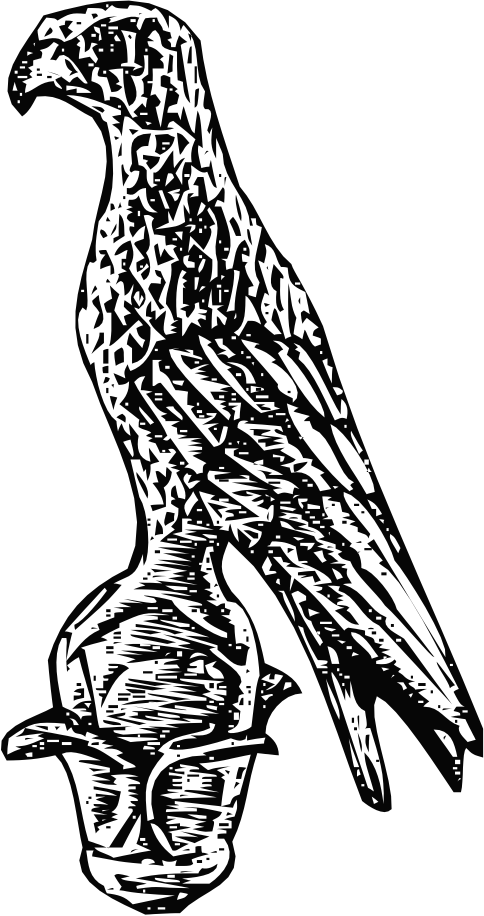
\includegraphics[width=0.35\linewidth]{uoi_logo}
\end{minipage}
\begin{minipage}{0.38\textwidth}
\begin{center}
{\normalfont\normalsize\scshape University of Ioannina}\\[0.7mm]
{\normalfont\normalsize\scshape School of Sciences}\\[0.7mm]
{\normalfont\normalsize\scshape Department of Physics}\\[0.7mm]
%{\normalfont\normalsize\scshape Section of Theoretical Physics}\\[0.7mm]
\end{center}
\end{minipage}
\begin{minipage}{0.1\textwidth}
    \quad
\end{minipage}
\begin{minipage}{0.19\textwidth}

\includegraphics[width=0.75\linewidth]{uoi_physics_logo}
\end{minipage}
%
\\ \vspace*{20mm}
%
\rule[0.5ex]{\linewidth}{2pt}\vspace*{-\baselineskip}\vspace*{2.5pt}
\rule[0.5ex]{\linewidth}{1pt}\\[2mm]
{\normalfont\LARGE\scshape Quantum Information Theory}\\[4mm]
%{\normalfont\Large\scshape of}\\[3mm]
{\normalfont\Large\scshape Algebraic and Physical Aspects}
\rule[0.5ex]{\linewidth}{1pt}\vspace*{-\baselineskip}\vspace{3.5pt}
\rule[0.5ex]{\linewidth}{2pt}\\
\vspace{12mm}
{\normalfont\itshape Lecture notes by}\\[1mm]
{\normalfont\Large\scshape Lampros Trifyllis}\\
\vspace{7mm}
{\normalfont\itshape for the undergraduate course on}\\[1mm]
{\normalfont\Large\scshape Quantum Theory of Information}
\vfill
{\large Ioannina 2026}
\\
{\normalsize [Draft date: \today]}
\end{center}
\end{adjustwidth*}
\end{titlingpage}


\chapter*{$\quad$}
%\chapter*{Dedication}

\thispagestyle{empty}

\epigraphfontsize{\small\itshape}

\epigraph{``Nature isn't classical, dammit,\\
and if you want to make a simulation of nature,\\
you'd better make it quantum mechanical\ldots'''}
%and by golly it's a wonderful problem,\\
%because it doesn't look so easy.''}
{--- \textup{Richard Feynman}}


% \openany % if the Acknowledgements take a second page consider putting it left and right
%\include{chapters/acknowledgements}

%\chapter*{Abstract}

In these lecture notes, we consider the foundational principles of Quantum Information Theory, the
interdisciplinary framework governing the storage, processing, and transmission of information via
quantum systems. The material is pedagogically divided into two conceptually distinct regimes. In
Part I, we establish the theoretical baseline of idealized, isolated quantum systems, focusing on
the paradigm shift from classical Boolean logic to the reversible, unitary evolution of quantum
states. Within this framework, we formalize the mathematical description of the quantum bits, or
qubits, superposition and entanglement within finite-dimensional Hilbert spaces. This serves as the
mathematical basis for defining fundamental quantum circuits, communication protocols and canonical
algorithms. In Part II, we extend the formalism beyond perfectly isolated systems, detailing the
transition from pure mathematical abstraction to the physical reality of open quantum systems. We
employ density matrices to model environmental coupling, quantum noise, and decoherence, and we
analyze the von Neumann entropy and the thermodynamics of information. Because of the inherent
fragility of these physical states, we focus on the necessity of quantum error-correction protocols.
Finally, we map this theoretical formalism to active experimental architectures defining the noisy
intermediate-scale quantum (NISQ) era, analyzing the physical realization of quantum computers using
superconducting circuits, trapped ions, and topological qubits.


\tableofcontents*
\clearpage
% \listoffigures
% \clearpage
% \listoftables
% \clearpage

\pagestyle{myheadings}

% \openright % if openany was used in the pre-matter use openright for the main-matter

%\include{chapters/preface}


% Main matter
\mainmatter

\chapterstyle{madsen}
\pagestyle{Ruled}

\part[Closed systems]{Closed systems}
\label{part:closedsystems}
\thispagestyle{empty}

% Individual chapters
%\input{chapters/chapter-01}


% Appendices

% Back matter
%\backmatter

%\chapterstyle{wilsondob}
%\pagestyle{myheadings}

% Bibliography
%\printbibliography[title=References]

\end{document}
